\documentclass[../main2.tex]{subfiles}
\begin{document}
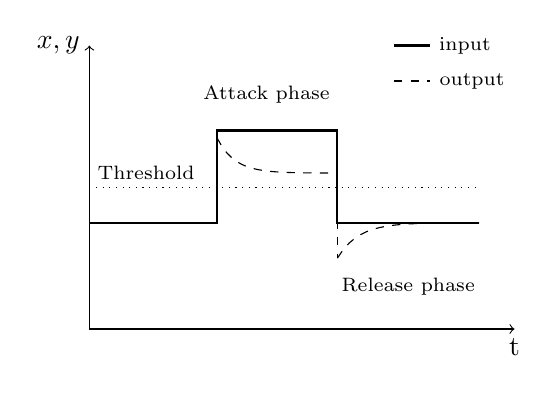
\begin{tikzpicture}[scale=0.9,baseline={(0,0)}]

%AXES
% horizontal axis
\draw[->] (0,0) -- (6,0) node[anchor=north] {t};
% vertical axis
\draw[->] (0,0) -- (0,4) node[anchor=east] {$x, y$};

%GRAPH
%input
\draw[thick] (0,1.5) -- (1.8,1.5) -- (1.8,2.8) -- (3.5,2.8) -- (3.5,1.5) -- (5.5,1.5);
%output
\draw[dashed,domain=1.8:3.5] plot (\x,{2.2+0.5*exp(-(\x-1.8)/0.25)});
\draw[dashed] (3.5, 2) -- (3.5, 1);
\draw[dashed,domain=3.5:5.5] plot (\x,{1.5-0.5*exp(-(\x-3.5)/0.3)});

%LABES
%threshold
\draw[dotted] (0,2) -- (5.5,2);
\draw(0.8,2.2) node{{\scriptsize Threshold}};

\draw(2.5, 3.3) node{{\scriptsize Attack phase}};
\draw(4.5,0.6) node{{\scriptsize Release phase}};

%legend
\draw[thick] (4.3,4) -- (4.8,4);
\draw(5.3, 4) node{{\scriptsize input}};

\draw[dashed] (4.3,3.5) -- (4.8,3.5);
\draw(5.4, 3.5) node{{\scriptsize output}};

\end{tikzpicture}
\end{document}
